% ------------------------------------------------------------------------------
% 6.1. ANÁLISIS DE LA ARQUITECTURA
% ------------------------------------------------------------------------------
\subsection{6.1. Análisis de la Arquitectura}\label{sec:cap6_arquitectura}

% [PENDIENTE]: Redactar el análisis de la arquitectura.

\subsubsection{6.1.1. Identificación de Paquetes}\label{sec:cap6_identificacion_paquetes}

% [PENDIENTE]: Identificar los paquetes de análisis del sistema.

\subsubsection{6.1.2. Relación de Paquetes}\label{sec:cap6_relacion_paquetes}

% [PENDIENTE]: Describir las dependencias entre paquetes.

\subsubsection{6.1.3. Encapsulamiento de Casos de Uso por Paquetes}\label{sec:cap6_encapsulamiento_cu}

% [PENDIENTE]: Redactar la introducción del encapsulamiento (criterio de agrupación de los casos de uso).

Las Figuras~\ref{fig:enc_cuentas}, \ref{fig:enc_convocatoria}, \ref{fig:enc_preseleccion}, \ref{fig:enc_auditoria}, \ref{fig:enc_becados} y~\ref{fig:enc_reportes} muestran el encapsulamiento de los casos de uso en cada uno de los seis paquetes de análisis del sistema.

El paquete Cuentas y Acceso encapsula los casos de uso CU-01, CU-14 y CU-15, como se muestra en la Figura~\ref{fig:enc_cuentas}.

\begin{figure}[H]
\caption{Encapsulamiento de casos de uso del paquete Cuentas y Acceso}
\label{fig:enc_cuentas}
\centering
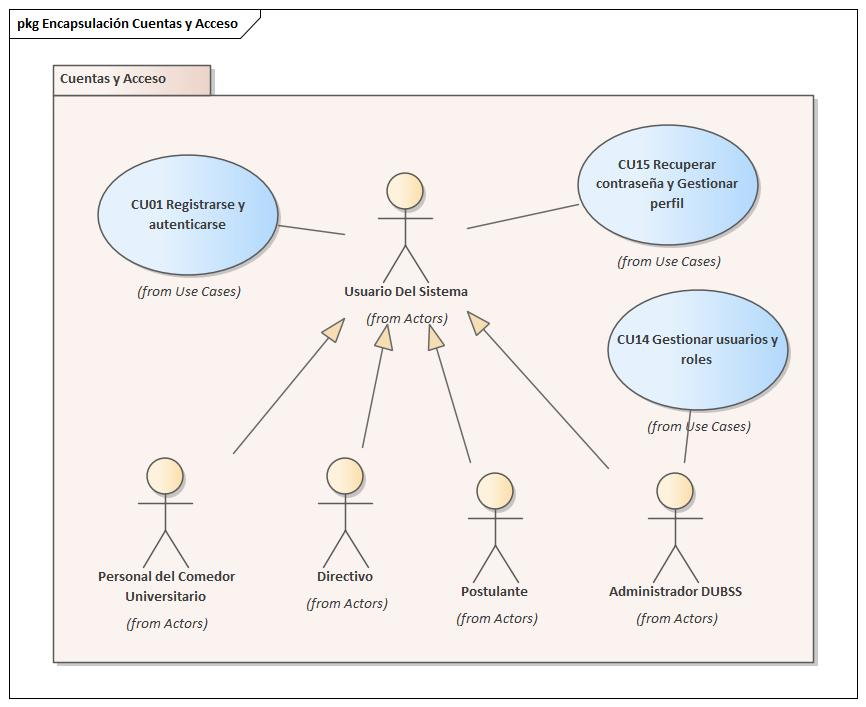
\includegraphics[width=\textwidth,height=0.85\textheight,keepaspectratio]{images/21_Encapsulamiento_Cuentas_Acceso.jpg}

\smallskip
\noindent\raggedright\textit{Nota.} Elaboración propia.
\end{figure}

El paquete Convocatoria y Postulación encapsula los casos de uso CU-02, CU-04, CU-13, CU-16, CU-17 y CU-18, como se muestra en la Figura~\ref{fig:enc_convocatoria}.

\begin{figure}[H]
\caption{Encapsulamiento de casos de uso del paquete Convocatoria y Postulación}
\label{fig:enc_convocatoria}
\centering
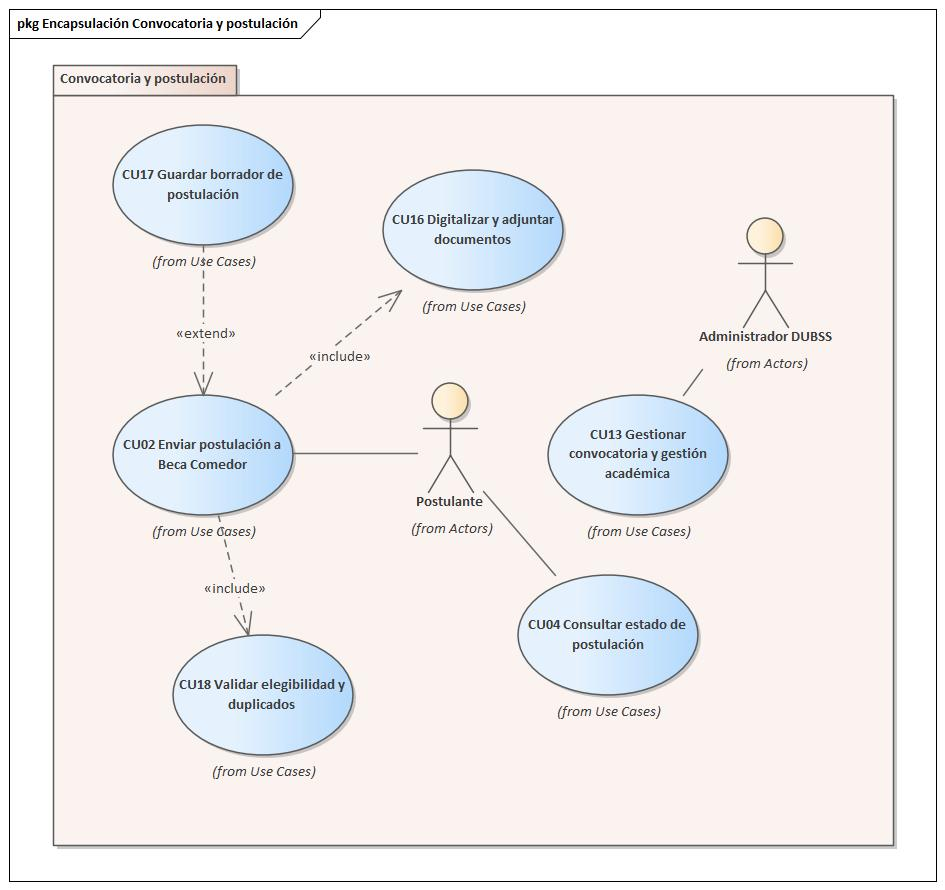
\includegraphics[width=\textwidth,height=0.85\textheight,keepaspectratio]{images/22_Encapsulamiento_Convocatoria_Postulacion.jpg}

\smallskip
\noindent\raggedright\textit{Nota.} Elaboración propia.
\end{figure}

El paquete Preselección con IA encapsula los casos de uso CU-03 y CU-26, como se muestra en la Figura~\ref{fig:enc_preseleccion}.

\begin{figure}[H]
\caption{Encapsulamiento de casos de uso del paquete Preselección con IA}
\label{fig:enc_preseleccion}
\centering
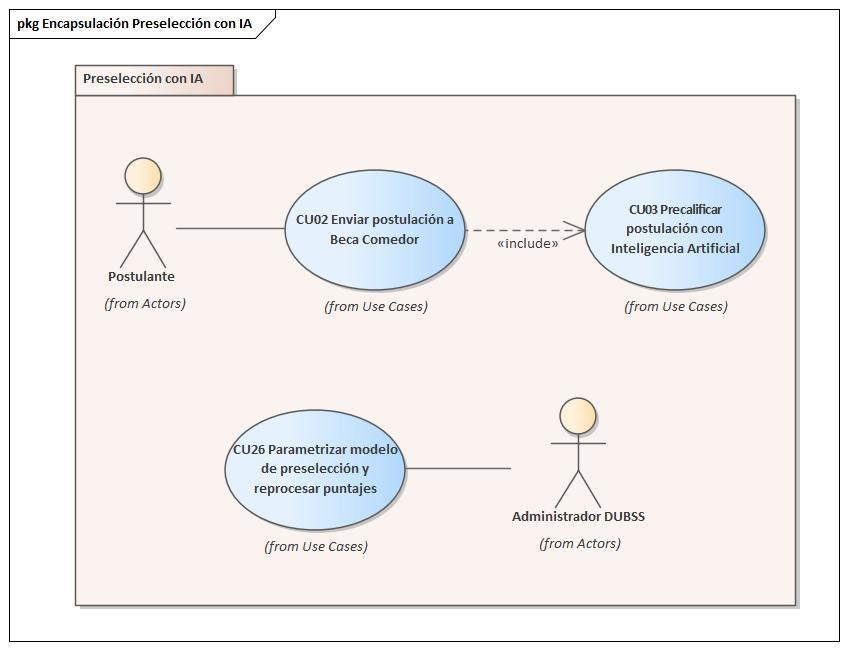
\includegraphics[width=\textwidth,height=0.85\textheight,keepaspectratio]{images/23_Encapsulamiento_Preseleccion_IA.jpg}

\smallskip
\noindent\raggedright\textit{Nota.} Elaboración propia.
\end{figure}

El paquete Auditoría y Adjudicación encapsula los casos de uso CU-05, CU-06, CU-07, CU-08, CU-19, CU-20, CU-21 y CU-22, como se muestra en la Figura~\ref{fig:enc_auditoria}.

\begin{figure}[H]
\caption{Encapsulamiento de casos de uso del paquete Auditoría y Adjudicación}
\label{fig:enc_auditoria}
\centering
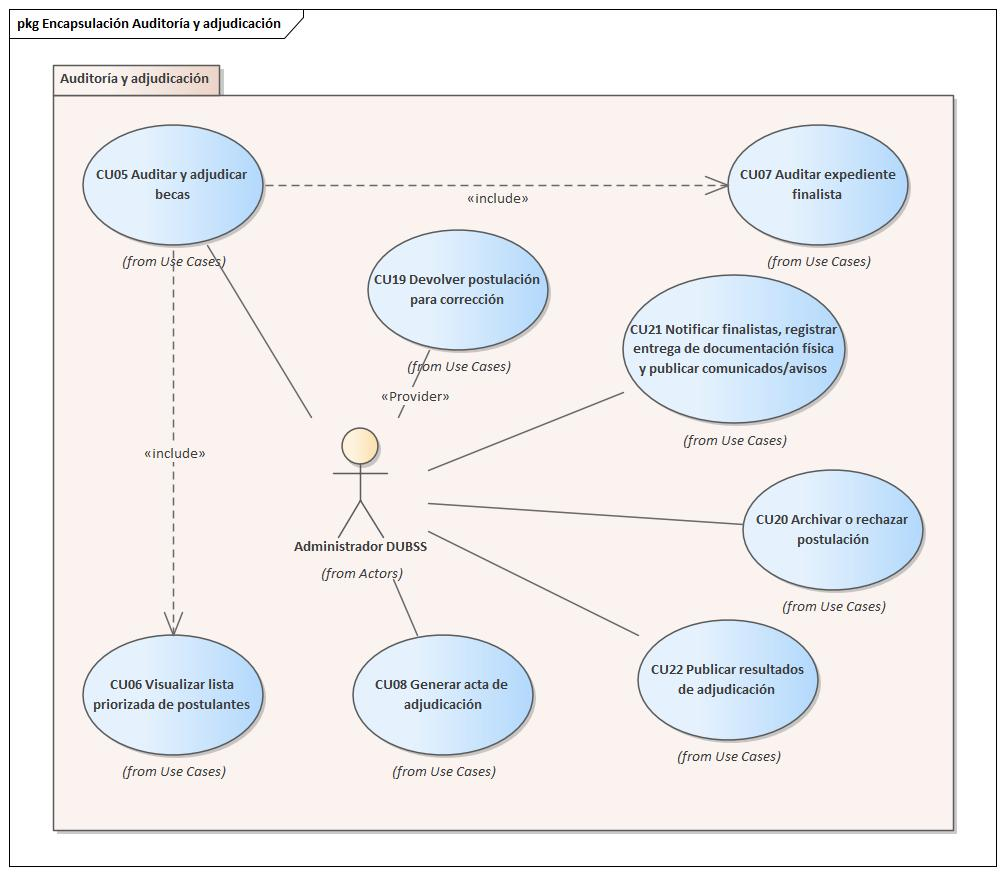
\includegraphics[width=\textwidth,height=0.85\textheight,keepaspectratio]{images/24_Encapsulamiento_Auditoria_Adjudicacion.jpg}

\smallskip
\noindent\raggedright\textit{Nota.} Elaboración propia.
\end{figure}

El paquete Becados y Asistencia encapsula los casos de uso CU-09, CU-10, CU-11, CU-23 y CU-24, como se muestra en la Figura~\ref{fig:enc_becados}.

\begin{figure}[H]
\caption{Encapsulamiento de casos de uso del paquete Becados y Asistencia}
\label{fig:enc_becados}
\centering
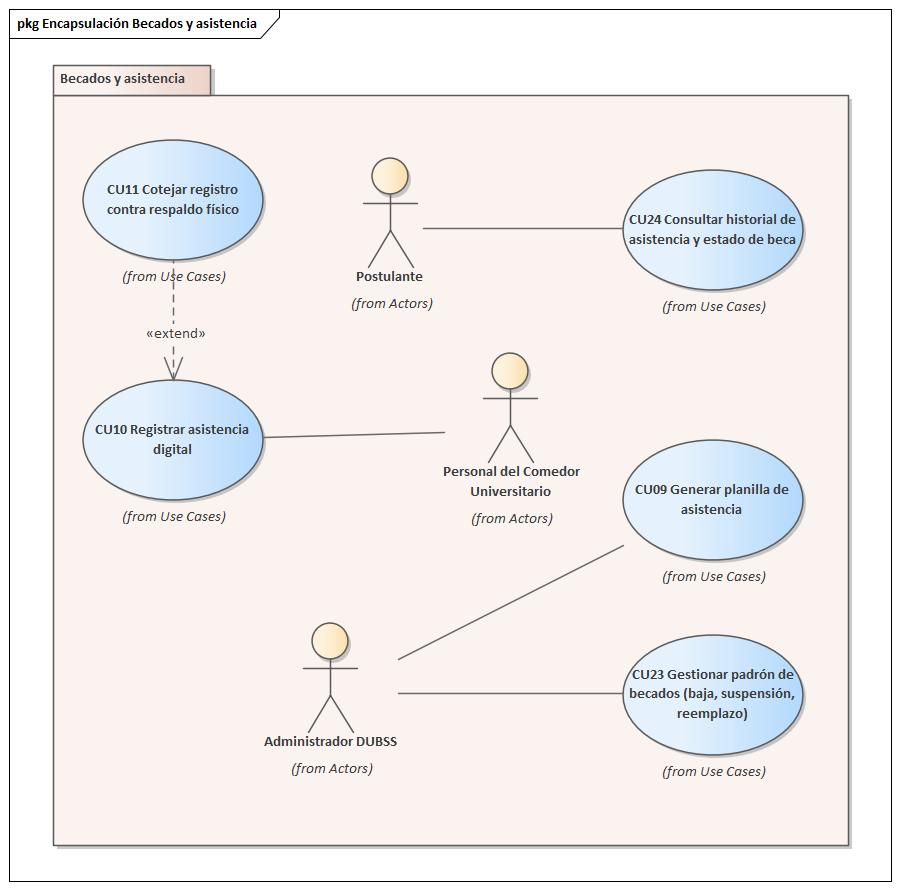
\includegraphics[width=\textwidth,height=0.85\textheight,keepaspectratio]{images/25_Encapsulamiento_Becados_Asistencia.jpg}

\smallskip
\noindent\raggedright\textit{Nota.} Elaboración propia.
\end{figure}

El paquete Reportes y Trazabilidad encapsula los casos de uso CU-12 y CU-25, como se muestra en la Figura~\ref{fig:enc_reportes}.

\begin{figure}[H]
\caption{Encapsulamiento de casos de uso del paquete Reportes y Trazabilidad}
\label{fig:enc_reportes}
\centering
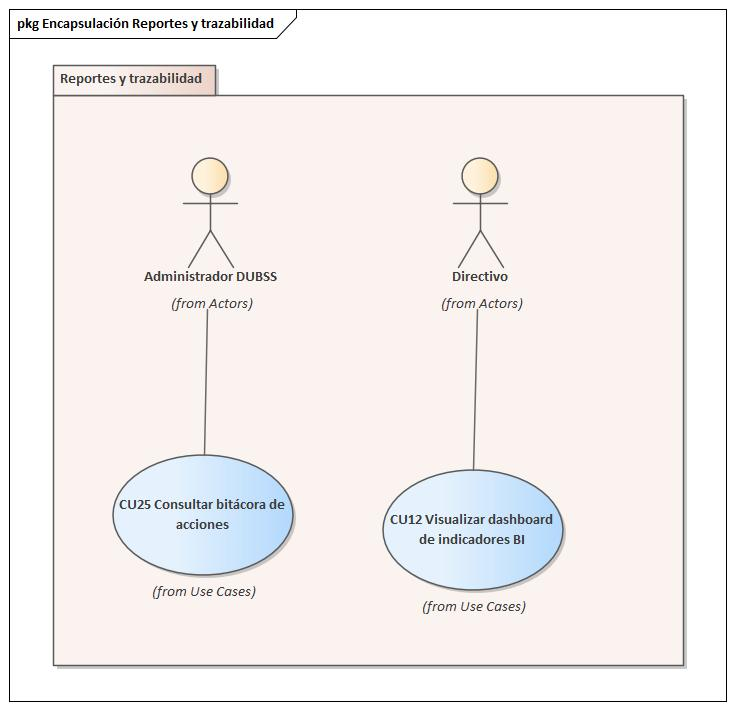
\includegraphics[width=\textwidth,height=0.85\textheight,keepaspectratio]{images/26_Encapsulamiento_Reportes_Trazabilidad.jpg}

\smallskip
\noindent\raggedright\textit{Nota.} Elaboración propia.
\end{figure}
